% !TeX root = ../main/main.tex
\documentclass[../main/main.tex]{subfiles}

\begin{document}
\espacio
  En este capítulo se muestran los resultados obtenidos de la ejecución del algoritmo AES Rijndael en CPU y GPU, así como la comparación de tiempos en ambos ambientes de investigación.

  \section{Paralelización del algoritmo AES Rijndael}

    Para la ejecución del algoritmo se utilizó el script en el entorno Python que se muestra en el Anexo \ref{anexo:script_aes_original}, mismo que fue desarrollado por Pablo Caro en Septiembre del año 2013.

    Este algoritmo fue modificado para la ejecución de sus funciones en paralelo mediante la librería Numba que cuenta con soporte para GPU CUDA, las modificaciones se muestran en el Anexo \ref{anexo:script_aes_modificado}.

    El entorno de trabajo se detalla en la sección [\ref{limites_alcances}] referente a Límites y Alcances.

    El tamaño de bloque a cifrar fue de 128 bits, lo que elimina el tiempo de ejecución de la operación de padding o el del recorte en sub-bloques.

    Los tiempos de cifrado y descifrado fueron tomados de acuerdo a las longitudes de clave estándar que son: 128, 192 y 256 bits. El proceso se ejecutó un total 1000 veces por cada longitud de clave. Cada proceso generó una muestra cuyo resultado generó un promedio de la diferencia de tiempos de ejecución entre CPU y GPU.

    \subsection{Comparación de tiempos de ejecución}

      \subsubsection{Cifrado con llave de 128 bits}

        \begin{figure}[H]
          \centering
          \caption{Cifrado con llave de 128 bits para un total de 1000 muestras}
          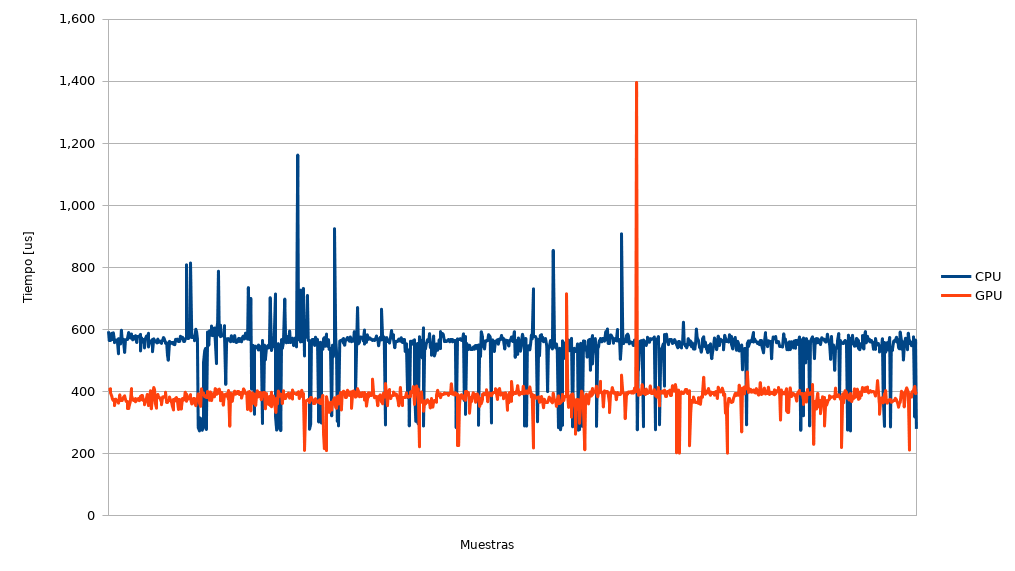
\includegraphics[width=15cm, keepaspectratio]{marco_teorico/cifrado_128_bits.png}
          \caption*{\textbf{Fuente:} Elaboración propia}
        \end{figure}

        Tiempo promedio de ejecución del algoritmo en CPU:

        \vspace{-0.7cm}\begin{equation}
          \overline{t_{CPU}} = 545.33\mu s
        \end{equation}

        Tiempo promedio de ejecución del algoritmo en CPU:

        \vspace{-0.7cm}\begin{equation}
          \overline{t_{GPU}} = 382.99\mu s
        \end{equation}

        Aceleración del algoritmo ejecutado en GPU respecto a la ejecución en CPU:

        \vspace{-0.7cm}\begin{equation}
          \frac{\overline{t_{CPU}}}{\overline{t_{GPU}}} = \frac{545.33\mu s}{382.99\mu s} = 1.42x
        \end{equation}

        Por tanto, la ejecución del algoritmo de cifrado en GPU es 1.42 veces más rápido que la ejecución en CPU, para un tamaño de llave de 128 bits.

      \subsubsection{Cifrado con llave de 192 bits}

        \begin{figure}[H]
          \centering
          \caption{Cifrado con llave de 192 bits para un total de 1000 muestras}
          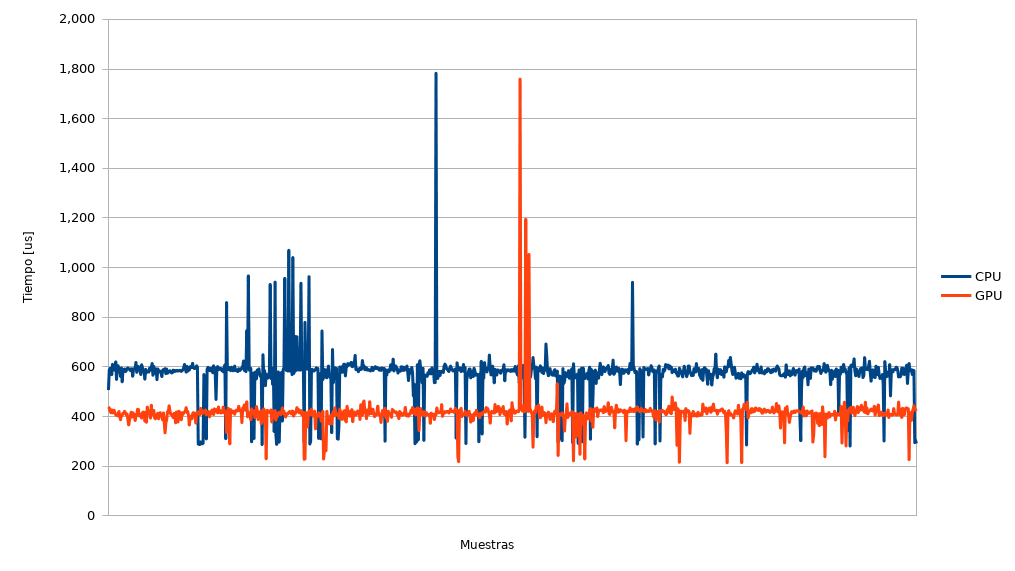
\includegraphics[width=15cm, keepaspectratio]{marco_teorico/cifrado_192_bits.png}
          \caption*{\textbf{Fuente:} Elaboración propia}
        \end{figure}

        Tiempo promedio de ejecución del algoritmo en CPU:

        \vspace{-0.7cm}\begin{equation}
          \overline{t_{CPU}} = 571.27\mu s
        \end{equation}

        Tiempo promedio de ejecución del algoritmo en CPU:

        \vspace{-0.7cm}\begin{equation}
          \overline{t_{GPU}} = 412.92\mu s
        \end{equation}

        Aceleración del algoritmo ejecutado en GPU respecto a la ejecución en CPU:

        \vspace{-0.7cm}\begin{equation}
          \frac{\overline{t_{CPU}}}{\overline{t_{GPU}}} = \frac{571.27\mu s}{412.92\mu s} = 1.38x
        \end{equation}

        Por tanto, la ejecución del algoritmo de cifrado en GPU es 1.38 veces más rápido que la ejecución en CPU, para un tamaño de llave de 192 bits.

      \subsubsection{Cifrado con llave de 256 bits}

        \begin{figure}[H]
          \centering
          \caption{Cifrado con llave de 256 bits para un total de 1000 muestras}
          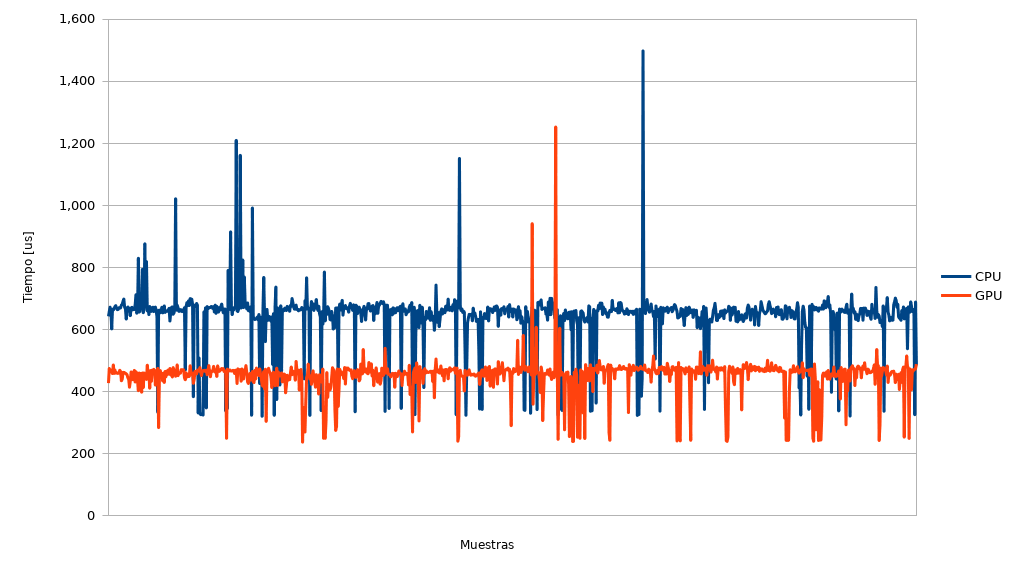
\includegraphics[width=15cm, keepaspectratio]{marco_teorico/cifrado_256_bits.png}
          \caption*{\textbf{Fuente:} Elaboración propia}
        \end{figure}

        Tiempo promedio de ejecución del algoritmo en CPU:

        \vspace{-0.7cm}\begin{equation}
          \overline{t_{CPU}} = 641.68\mu s
        \end{equation}

        Tiempo promedio de ejecución del algoritmo en CPU:

        \vspace{-0.7cm}\begin{equation}
          \overline{t_{GPU}} = 451.16\mu s
        \end{equation}

        Aceleración del algoritmo ejecutado en GPU respecto a la ejecución en CPU:

        \vspace{-0.7cm}\begin{equation}
          \frac{\overline{t_{CPU}}}{\overline{t_{GPU}}} = \frac{641.68\mu s}{451.16\mu s} = 1.42x
        \end{equation}

        Por tanto, la ejecución del algoritmo de cifrado en GPU es 1.42 veces más rápido que la ejecución en CPU, para un tamaño de llave de 256 bits.

      \subsubsection{Descifrado con llave de 128 bits}

        \begin{figure}[H]
          \centering
          \caption{Descifrado con llave de 128 bits para un total de 1000 muestras}
          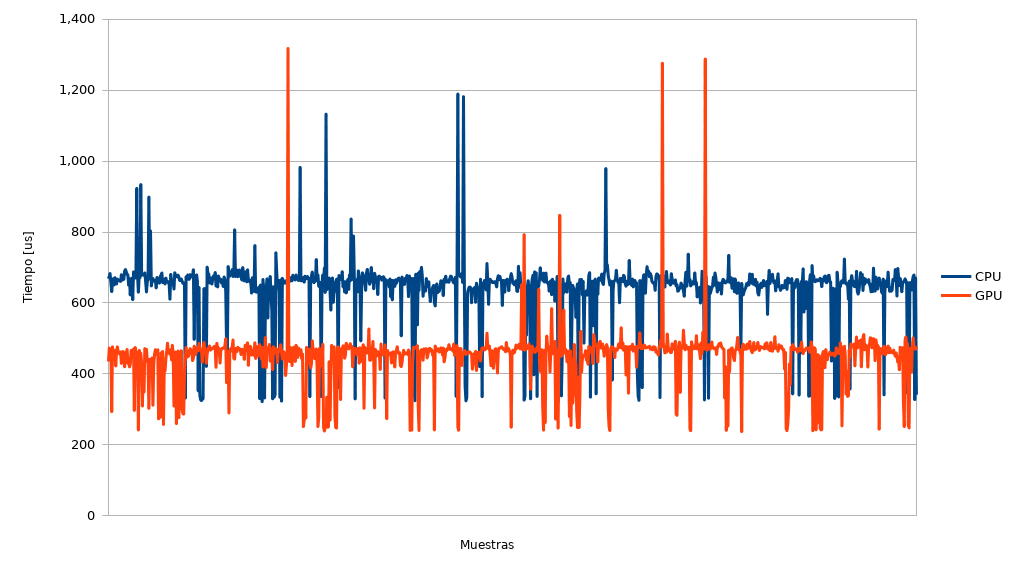
\includegraphics[width=15cm, keepaspectratio]{marco_teorico/descifrado_128_bits.png}
          \caption*{\textbf{Fuente:} Elaboración propia}
        \end{figure}

        Tiempo promedio de ejecución del algoritmo en CPU:

        \vspace{-0.7cm}\begin{equation}
          \overline{t_{CPU}} = 640.24\mu s
        \end{equation}

        Tiempo promedio de ejecución del algoritmo en CPU:

        \vspace{-0.7cm}\begin{equation}
          \overline{t_{GPU}} = 449.68\mu s
        \end{equation}

        Aceleración del algoritmo ejecutado en GPU respecto a la ejecución en CPU:

        \vspace{-0.7cm}\begin{equation}
          \frac{\overline{t_{CPU}}}{\overline{t_{GPU}}} = \frac{640.24\mu s}{449.68\mu s} = 1.42x
        \end{equation}

        Por tanto, la ejecución del algoritmo de descifrado en GPU es 1.42 veces más rápido que la ejecución en CPU, para un tamaño de llave de 128 bits.

      \subsubsection{Descifrado con llave de 192 bits}

        \begin{figure}[H]
          \centering
          \caption{Descifrado con llave de 192 bits para un total de 1000 muestras}
          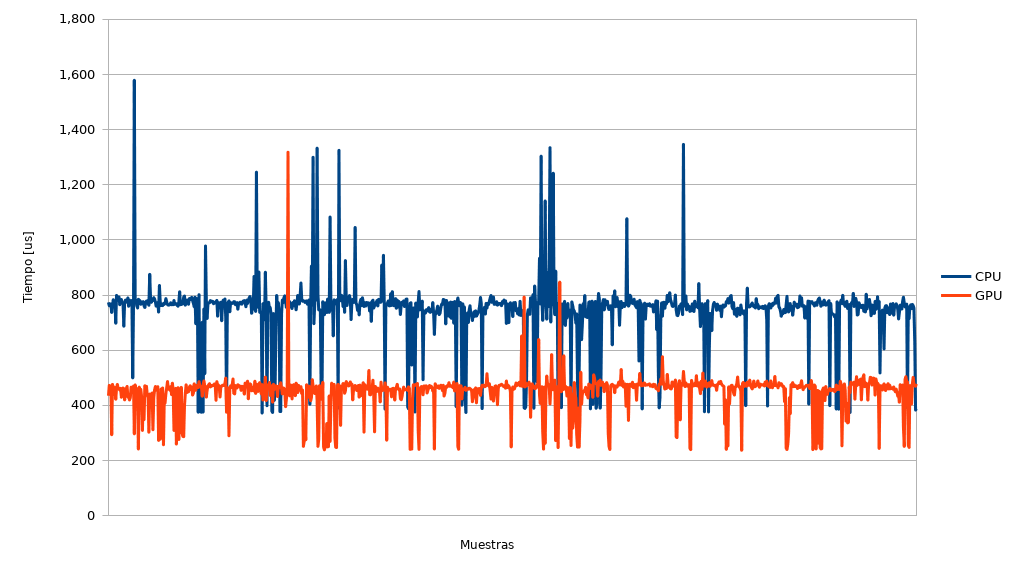
\includegraphics[width=15cm, keepaspectratio]{marco_teorico/descifrado_192_bits.png}
          \caption*{\textbf{Fuente:} Elaboración propia}
        \end{figure}

        Tiempo promedio de ejecución del algoritmo en CPU:

        \vspace{-0.7cm}\begin{equation}
          \overline{t_{CPU}} = 745.25\mu s
        \end{equation}

        Tiempo promedio de ejecución del algoritmo en CPU:

        \vspace{-0.7cm}\begin{equation}
          \overline{t_{GPU}} = 448.18\mu s
        \end{equation}

        Aceleración del algoritmo ejecutado en GPU respecto a la ejecución en CPU:

        \vspace{-0.7cm}\begin{equation}
          \frac{\overline{t_{CPU}}}{\overline{t_{GPU}}} = \frac{745.25\mu s}{448.18\mu s} = 1.66x
        \end{equation}

        Por tanto, la ejecución del algoritmo de descifrado en GPU es 1.66 veces más rápido que la ejecución en CPU, para un tamaño de llave de 192 bits.

      \subsubsection{Descifrado con llave de 256 bits}

        \begin{figure}[H]
          \centering
          \caption{Descifrado con llave de 256 bits para un total de 1000 muestras}
          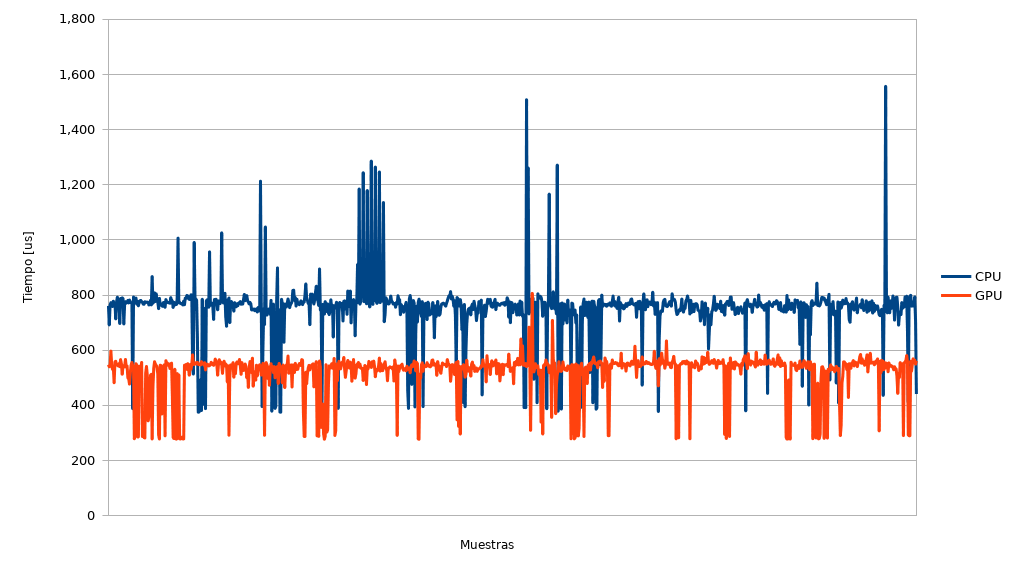
\includegraphics[width=15cm, keepaspectratio]{marco_teorico/descifrado_256_bits.png}
          \caption*{\textbf{Fuente:} Elaboración propia}
        \end{figure}

        Tiempo promedio de ejecución del algoritmo en CPU:

        \vspace{-0.7cm}\begin{equation}
          \overline{t_{CPU}} = 748.93\mu s
        \end{equation}

        Tiempo promedio de ejecución del algoritmo en CPU:

        \vspace{-0.7cm}\begin{equation}
          \overline{t_{GPU}} = 520.02\mu s
        \end{equation}

        Aceleración del algoritmo ejecutado en GPU respecto a la ejecución en CPU:

        \vspace{-0.7cm}\begin{equation}
          \frac{\overline{t_{CPU}}}{\overline{t_{GPU}}} = \frac{748.93\mu s}{520.02\mu s} = 1.44x
        \end{equation}

        Por tanto, la ejecución del algoritmo de descifrado en GPU es 1.44 veces más rápido que la ejecución en CPU, para un tamaño de llave de 256 bits.

    \subsection{Cálculo de la aceleración del algoritmo ejecutado en GPU con respecto a la ejecución en CPU}

        De acuerdo a los resultados mostrados anteriormente, se puede calcular el promedio de aceleración del algoritmo de cifrado ejecutado en GPU con respecto a la ejecución en CPU.

        \vspace{-0.7cm}\begin{equation}
          \frac{1.42 + 1.38 + 1.42}{3} = 1.41x
        \end{equation}

        De igual manera se puede calcular el promedio de aceleración del algoritmo de descifrado ejecutado en GPU con respecto a la ejecución en CPU.

        \vspace{-0.7cm}\begin{equation}
          \frac{1.42 + 1.66 + 1.44}{3} = 1.51x
        \end{equation}

\end{document}